\section{Funktionale Anforderungen}

\subsection{Programmausführung}

\label{subsec:programmausfuehrung}

	\begin{description}
		
		\item[/F010/] \textit{Programm beenden:}\par In der Projektansicht und der Projektübersicht ist die Möglichkeit gegeben, durch betätigen der "`Fenster schließen"' Schaltfläche (differiert je nach Betriebssystem), das Programm zu beenden. Vor dem endgültigen Schließen, wird eine Sicherheitsabfrage (ein Dialog mit Ja/Nein/Abbrechen Auswahlmöglichkeit) angezeigt, die dem Benutzer die Möglichkeit gibt, das Projekt zu speichern oder das Schließen des Projektes abzubrechen.
		
		\item[/F020/] \textit{Speicherverhalten:}\par Nach jedem Dialog ist die Möglichkeit gegeben, die aktuelle Änderung für die aktuelle Programmausführung zu übernehmen. Sollen Änderungen dauerhaft gesichert werden, muss die Schaltfläche "`Speichern"' in dem Bereich "`Projekt"' der Projektansicht betätigt werden. Dadurch, wird die Projektkonfigurationsdatei neu generiert und in dem Projektverzeichnis (siehe Kapitel \ref{subsec:projektmanagement} gespeichert.)
		
		\item[/F030/] \textit{Automatische Anpassung der Größe der Bedienoberfläche:}\par Das Programm positioniert automatisch seine Bedienelemente, in Abhängigkeit zur Auflösung des Programmfensters.
		
		\item[/F040/] \textit{Automatisches durchsuchen des Projektverzeichnisses:}\par Bei Programmstart, wird in dem Projektverzeichnis des Programms nach Projektkonfigurationsdateien gesucht. Auf der Basis dieser Datensätze wird eine Projektliste generiert, die in einer Projektübersicht, nach absteigendem Bearbeitungsdatum (aktuelles zuerst), sortiert angezeigt werden. Zudem wird das Datum anders formatiert dargestellt als der Projektname.
		
		\item[/F050/] \textit{Besondere Formatierung markierter Listeneinträge:}\par Ist ein Listeneintrag markiert, so wird er durch eine andere Vorder- und Hintergrundfarbe von anderen Listeneinträgen abgehoben.

		\item[/F060/] \textit{Listen mit Scrollbalken versehen:}\par Hat eine Liste so viele Einträge, dass sie nicht mehr in die Anzeige passen, wird ein Scrollbalken aktiviert mit dem man sich alle Einträge anzeigen lassen kann.
		
		\item[/F065/] \textit{Lexikographisches Sortieren:}\par	Beim \gls{lexgraph}en Sortieren gilt allgemein im gesamten Programm, dass nach den java.text.Collator Rules von SUN, welche abhängig sind von Locale, sortiert wird.
		
		\item[/F070/] \textit{Namensvergabe Allgemein:}\par	Beim Ausfüllen von Textfeldern gilt allgemein im gesamten Programm es darf UTF8 ohne Steuerzeichen verwendet werden.
		
	\end{description}

\subsection{Projektmanagement}

\label{subsec:projektmanagement}
	
	\gls{tempX} verfügt über eine eingebaute Projektverwaltung, mit der der Benutzer beliebige Kombinationen von Bildmengen und Auswertungen verwalten kann. Es kann allerdings immer nur ein Projekt geöffnet sein, ein Wechsel in ein anderes Projekte während der Programmausführung ist möglich.\par Ein Projekt wird in einer Projektkonfigurationsdatei gespeichert, die sich in dem Projektverzeichnis von \gls{tempX} befindet. Dabei wird nicht der Name des Projekts als Name der Projektkonfigurationsdatei verwendet, sondern die Projekt-ID, die programmweit eindeutig sein muss.\par Um den Speicherort des Projektverzeichnisses zu ermitteln, wird die betriebssystemspezifische Variable in der das Benutzerverzeichnis des aktuellen Benutzers festgelegt ist abgefragt.\\ Ausgehend von diesem Verzeichnis, wird der Ordner "`\gls{tempX}\_projekte"' angelegt oder verwendet, falls er schon vorhanden ist.
	
	\begin{description}		
		
		%TODO Nach der Eingabe, werden für die Speicherung kritische Steuerzeichen erkannt und dem Benutzer die Möglichkeit gegeben, seine Eingabe zu korrigieren.
		\item[/F110/] \textit{Neues Projekt anlegen:}\par In der Projektübersicht ist die Möglichkeit gegeben, durch betätigen der Schaltfläche "`Projekt erstellen"', ein neues Projekt zu erstellen und ihm einen Namen zu geben.\par Dabei wird überprüft, ob dieser Projektname schon von einem anderen Projekt verwendet wird. Ist dies der Fall, kann der Benutzer einen neuen Namen eingeben. Dabei ist auch zu beachten, dass der Projektname zwischen einem und 255 Zeichen lang sein muss. \par Bei der Projektanlegung wird auch ein Erstellungsdatum erstellt (siehe Kapitel \ref{subsec:programmdaten} \textbf{/D20/}). Danach wird die Projektansicht gestartet, mit dem gerade erstellten Projekt (siehe Kapitel \ref{subsec:benutzerschnittstelle}). Zu beachten ist, dass ein Projekt erst nach der in Kapitel \ref{subsec:programmausfuehrung} beschriebenen Funktion \textbf{/F020/} dauerhaft verfügbar ist. 
		
		\item[/F120/] \textit{Projekt markieren:}\par Um eine Projekt zu markieren, muss man es in der Liste der Projekte, in dem Dialog aus \textbf{/F040/}, auswählen.
		
		\item[/F130/] \textit{Vorhandenes Projekt öffnen:}\par In der Projektübersicht ist die Möglichkeit gegeben, durch einen Doppelklick mit der linken Maustaste auf den Projektnamen eines bereits vorhanden Projektes oder durch markieren eines Projektes und betätigen der Schaltfläche "`Projekt öffnen"' (siehe Kapitel \ref{subsec:benutzerschnittstelle}) die Projektansicht zu starten.\par Die damit verbundenen Bildmengen und Auswertungen, welche in der demenstprechenden Projektkonfigurationsdatei gespeichert sind, werden nun verfügbar gemacht. Damit gemeint ist: 
			
			\begin{itemize}
				
				\item Das Einlesen von \gls{exif}-Parametern aller Bilder, die in den Bildmengen des Projekts definiert sind. Das Einlesen geschieht im Hintergrund, d.h. der Benutzer kann mit dem Programm interagieren, vollständige Funktionalität ist aber erst nach dem vollständigen Einlesen der \gls{exif}-Parameter gegeben.
				
				\item Anzeige der Bildmengen (siehe Kapitel \ref{subsec:bildmengenmgmt} \textbf{/F250/}).
				
				\item Anzeige der Auswertungen (siehe Kapitel \ref{subsec:auswertungsmgmt}).
				
				\item Anzeige aller Bilder der Bildmengen in dem Bereich "`Bildansicht"' und Markieren des ersten Bildes. Dadurch wird der Bereich "`\gls{exif}-Daten"' der Projektansicht, mit den \gls{exif}-Parametern dieses Bildes aktualisiert.
			
			\end{itemize}		
		
		\item[/F140/] \textit{Projekt kopieren:}\par In der Projektübersicht ist die Möglichkeit gegeben, ein markiertes Projekt mit allen in ihm definierten Daten, Bildmengen und Auswertungen zu kopieren und es unter neuem Namen und neuem Erstellungsdatum temporär zu definieren (siehe Kapitel \ref{subsec:projektmanagement} \textbf{/F110/}). Danach wird die Projektansicht gestartet, mit dem gerade kopierten Projekt (siehe Kapitel \ref{subsec:benutzerschnittstelle}). Zu beachten ist, dass ein Projekt erst nach der in Kapitel \ref{subsec:programmausfuehrung} beschriebenen Funktion \textbf{/F020/} dauerhaft verfügbar ist.
		
		\item[/F150/] \textit{Projekt entfernen:}\par In der Projektübersicht ist die Möglichkeit gegeben, bei einem markierten Projekt mit betätigen der Schaltfläche "`Projekt entfernen"' folgende Aktionen auszulösen:
			
			\begin{enumerate}
				
				\item Es wird eine Sicherheitsabfrage (ein Dialog mit Ja/Nein Auswahlmöglichkeit) angezeigt, die dem Benutzer die Möglichkeit gibt, das Entfernen abzubrechen.
				
				\item Das Projekt wird aus der Liste der Projekte, in der Projektübersicht, entfernt.
				
				\item Die Projektkonfigurationsdatei, wird in dem Projektverzeichnis gelöscht.
				
				\item Dem Benutzer wird eine Rückmeldung gegeben, ob das Entfernen erfolgreich war oder ob es einen Fehler gab.
			
			\end{enumerate}
	
		\item[/F160/] \textit{Projektbeschreibung hinzufügen:}\par In dem Feld "`Projektbeschreibung"' lässt sich das Projekt genauer spezifizieren. Erst nach Ausführung von \textbf{/F020/} ist dies dauerhaft möglich.
	
		\item[/F170/] \textit{Projekt wechseln:}\par Durch betätigen der Schaltfläche "`Wechseln"' in dem Bereich "`Projekt"' der Projektansicht, werden folgende Aktionen ausgelöst:
		
		\begin{enumerate}
				
				\item Es wird eine Sicherheitsabfrage (ein Dialog mit Ja/Nein/Abbrechen Auswahlmöglichkeit) angezeigt, die dem Benutzer die Möglichkeit gibt das Projekt zu speichern oder das Wechseln des Projektes abzubrechen.
				
				\item Das gerade geöffnete Projekt wird geschlossen.
				
				\item Die Projektansicht wird beendet.
				
				\item Die Projektübersicht wird gestartet.
			
			\end{enumerate}

		\item[/F180/] \textit{Projektnamen ändern:}\par Durch eine Neueingabe des Projektnamens im Projektnamenfeld des Bereichs "`Projekt"' in der Projektansicht, wird dem Projekt ein neuer Name vergeben. Dabei werden die Richtlinien bezüglich des Projektnamens aus \textbf{/F110/} angewandt.
	
	\end{description}

\subsection{Bildmengenmanagement}

\label{subsec:bildmengenmgmt}
	
	In einem Projekt, können Bildmengen verwaltet werden (siehe Kapitel \ref{sec:nichtfunktionale_anforderungen} \textbf{/NF020/}). Eine Bildmenge ist folgendermaßen definiert:
	
	\begin{itemize}
		
		\item Eine Bildmenge kann beliebig (im Rahmen der \textbf{/NF020/)} viele Verweise auf Bilder (im \gls{jpg}-Format) des verwendeten Dateisystems enthalten.
		
		\item Eine Bildmenge kann beliebig (im Rahmen der \textbf{/NF020/)} viele Verweise auf Verzeichnisse des verwendeten Dateisystems enthalten.
		
		\item Eine Bildmenge kann beliebig (im Rahmen der \textbf{/NF020/)} viele Verweise auf Bildmengen haben, die in dem Projekt definiert sind. Dabei ist zu beachten:
		
			\begin{itemize}
			
				\item Bei den Verweisen, darf es zu keinen Endlosverweisen führen (Bildmenge A ist in Bildmenge B und Bildmenge B ist in Bildmenge A).
				
				\item Wird eine Bildmenge entfernt, so werden alle Verweise auf diese Bildmenge ebenfalls entfernt.
			
			\end{itemize}
		
		\item Eine Bildmenge hat einen frei definierbaren und vom Projektkontext abhängigen eindeutigen Namen, der zwischen einem und 255 Zeichen lang sein muss.
		
		\item Eine Bildmenge wird über eine interne ID, die innerhalb eines Projekt eindeutig ist, identifiziert.
	
	\end{itemize}
	
Es ist außerdem zu beachten, dass bei einem Dateisystem- oder einem Datenspeicherstrukturwechsel die Verweise keine Gültigkeit mehr haben können und ein Neuanlegen dieser Verweise unumgänglich ist.\par Wird ein Projekt geöffnet, werden alle in der Projektkonfigurationsdatei definierten Bildmengen \gls{lexgraph} sortiert angezeigt. Die erste Bildmenge der Liste (falls vorhanden), wird dabei automatisch markiert.
	
	\begin{description}
		
		\item[/F210/] \textit{Anlegen einer neuen Bildmenge:}\par Durch betätigen der Schaltfläche "`Erstellen"' im Bereich "`Bildmengen"' der Projektansicht, wird ein Dialog geöffnet, der dem Benutzer die Möglichkeit gibt, der Bildmenge einen Namen zu geben.
		
		\item[/F220/] \textit{Markieren einer Bildmenge:}\par Um eine Bildmenge zu markieren, muss man sie in der Liste der Bildmengen, im Bereich "`Bildmengen"' der Projektansicht, auswählen. Dadurch wird der Bereich "`Inhalt"' der Projektansicht aktualisiert (siehe Kapitel \textbf{/F250/}).
		
		\item[/F230/] \textit{Hinzufügen von Bildern und Verzeichnissen zu einer vorhandenen Bildmenge:}\par Um diese Aktionen auszuführen, muss eine Bildmenge markiert sein. Das Hinzufügen kann über zwei Arten geschehen:
		
			\begin{itemize}
				
				\item Durch \gls{dragndrop} von Verzeichnissen und Bildern aus der grafischen Benutzerschnittstelle des Betriebssystems in den Bereich "`Inhalt"', einer markierten Bildmenge. 
				
				\item Durch betätigen der Schaltfläche "`Hinzufügen"' in dem Bereich "`Inhalt"' der Projektansicht einer markierten Bildmenge, wird ein Dialog mit Bildvorschau geöffnet, der dem Benutzer folgende Möglichkeiten gibt:
				
					\begin{itemize}
			
						\item Auswahl beliebig (im Rahmen der \textbf{/NF020/)} vieler Verzeichnisse, die einzeln als Pfade zum jeweiligen Verzeichnis in die Bildmenge übernommen werden. Ausgehend von diesen Verzeichnissen, wird rekursiv der Verzeichnisbaum nach Bilder im \gls{jpg}-Format durchsucht.
						
						\item Auswahl beliebig (im Rahmen der \textbf{/NF020/)} vieler Bilder im \gls{jpg}-Format, deren Pfade einzeln in die Bildmenge übernommen werden.
					
					\end{itemize}
				
				Der Dialog zeigt dabei nur Bilder im \gls{jpg}-Format oder Verzeichnisse an.
				
			\end{itemize}
		
		\item[/F240/] \textit{Hinzufügen von Bildmengen zu einer vorhandenen Bildmenge:}\par Das Hinzufügen kann nur per \gls{dragndrop} einer vorhanden Bildmenge aus dem Bereich "`Bildmengen"' der Projektansicht in den Bereich "`Inhalt"' der Projektansicht einer markierten Bildmenge erfolgen. Dabei wird die Definition von Bildmengen eingehalten (siehe Kapitel \ref{subsec:bildmengenmgmt}).
		
		\item[/F250/] \textit{Entfernen von Bildmengen:}\par Um diese Aktionen auszuführen, muss eine Bildmenge markiert sein. Durch betätigen der Schaltfläche "`Entfernen"', werden folgende Aktionen ausgelöst:
			
			\begin{enumerate}
			
				\item Es wird eine Sicherheitsabfrage (ein Dialog mit Ja/Nein Auswahlmöglichkeit) angezeigt, die dem Benutzer die Möglichkeit gibt, das Entfernen abzubrechen.
				
				\item Die Bildmenge wird aus der Liste der Bildmengen in dem Bereich "`Bildmengen"' der Projektansicht, entfernt.
				
				\item Es werden alle restlichen Bildmengen nach Verweisen auf diese Bildmenge durchsucht. Falls Verweise vorhanden sind, werden diese Verweise entfernt.
				
				\item Dem Benutzer wird eine Rückmeldung gegeben, ob das Entfernen erfolgreich war oder ob es einen Fehler gab.
				
				\item Nach dem Entfernen, ist die erste Bildmenge (falls vorhanden) in der Liste markiert.
			
			\end{enumerate}

		\item[/F260/] \textit{Aufbau der Inhaltsliste:}\par Ist eine Bildmenge markiert, wird in dem Bereich "`Inhalt"' der Proektansicht die Liste mit dem Inhalt der Bildmenge aktualisiert. Die Liste wird dabei blockweise nach folgendem Schema aufgebaut:
		
			\begin{enumerate}
			
				\item Mit der Bildmenge verknüpfte Bildmengen, \gls{lexgraph} sortiert.
			
				\item Mit der Bildmenge verknüpfte Verweise auf Verzeichnise, \gls{lexgraph} sortiert.
				
				\item Mit der Bildmenge verknüpfte Verweise auf Bilder, \gls{lexgraph} sortiert.
				
			\end{enumerate}
			
			Jeder Block ist dabei mit einer unterschiedlichen Textfarbe formatiert.
		
		\item[/F270/] \textit{Markieren eines Eintrags der Inhaltsliste:}\par Um einen Eintrag der Inhaltsliste zu markieren, muss man ihn in der Liste der Inhalte in dem Bereich "`Inhalt"' der Projektansicht, auswählen.
		
		\item[/F280/] \textit{Entfernen von Inhalten aus der Inhaltsliste:}\par Um diese Aktionen auszuführen, muss ein Eintrag in der Inhaltsliste markiert sein. Durch betätigen der Schaltfläche "`Entfernen"' in dem Bereich "`Inhalt"' der Projektansicht, werden folgende Aktionen ausgelöst:
			
			\begin{enumerate}
			
				\item Es wird eine Sicherheitsabfrage (ein Dialog mit Ja/Nein Auswahlmöglichkeit) angezeigt, die dem Benutzer die Möglichkeit gibt, das Entfernen abzubrechen.
				
				\item Der Eintrag wird aus der Inhaltsliste in dem Bereich "`Inhalte"' der Projektansicht, entfernt.
				
				\item Dem Benutzer wird eine Rückmeldung gegeben, ob das Entfernen erfolgreich war oder ob es einen Fehler gab.
				
				\item Nach dem Entfernen, ist der erste Eintrag (falls vorhanden) in der Liste markiert.
			
			\end{enumerate}
		
		\item[/F290/] \textit{Aktivieren/Deaktivieren von Bildern in der Bilderliste einer Bildermenge:}\par Standardmäßig sind aller Bilder in der Bilderliste einer Bildermenge aktiviert. Durch klicken auf eine Checkbox vor einem Bild, wird der Status abwechselnd von aktiv auf inaktiv oder inaktiv auf aktiv gesetzt. Aktiv bedeutet, dass in einer Checkbox vor dem Bild ein Haken gesetzt ist. Ist ein Bild im Status inaktiv, ist die Checkbox vor dem Bild leer und der Bildname ist ausgegraut.

		\item[/F295/] \textit{Anzeige von Exif-Parametern bei Bildmarkierung:}\par Wird durch Mausklick ein Bild in der Bildliste ausgewählt, wird der Bereich "`\gls{exif}-Daten"' der Projektansicht, mit den \gls{exif}-Parametern dieses Bildes aktualisiert.
		
	\end{description}

\subsection{Diagrammmanagement}

\label{subsec:diagrammmgmt}

	\gls{tempX} beherrscht verschiedene Diagrammtypen, welche im folgenden genannt sind:
	\newpage
	\begin{description}

		\item[/F310/] \textit{Tabelle:}\par 
		
			\begin{figure}[H]
				\centering
				\fbox{
					\begin{minipage}{13 cm}
						\centering
						\resizebox{13 cm}{!} {
\begin{tabular}{|c|c|c|c|c|c|c|}
\hline  Name & Manufacturer & Date and Time & FNumber & Exposure Time & Flash \\ 
\hline  DSC00601.JPG & Sony Ericsson   & 2009:11:07 00:27:48  & f/2,8 & 1/1000 & False\\ 
\hline  DSC00602.JPG & Sony Ericsson & 2009:11:06 10:27:26 & f/2,8  & 1/1600 & False \\ 
\hline  DSC00606.JPG & Sony Ericsson & 2009:11:06 12:35:59 & f/2,8  & 1/800 & False \\ 
\hline  SDC16734.JPG & Samsung Techwin & 2009:11:05 00:59:01   & f/7,0 & 1/250 & False\\ 
\hline  SDC16742.JPG & Samsung Techwin & 2009:11:06 05:52:36   & f/7,1 & 1/250 & False\\ 
\hline 
\end{tabular} 

}
						\caption{Ansicht einer tabellarischen Auswertung}
						\label{diag:tabelle}
					\end{minipage}  
				}    		
			\end{figure}			
			Die Tabelle stellt alle auszuwertenden \gls{exif}-Daten mit Dateinamen tabellarisch dar (siehe Kapitel \ref{subsec:auszuwertendedaten}). Dabei wird \gls{lexgraph} nach dem Dateinamen sortiert. Die Tabelle kann als \gls{jpg} via eines Dateidialogs exportiert werden.

		\item[/F320/] \textit{2D Histogramm:}\par 
		
			\begin{figure}[H]
				\centering
				\fbox{
					\begin{minipage}{13 cm}
						\centering						
						% Generated with LaTeXDraw 2.0.2
% Tue Nov 17 01:27:38 CET 2009
% \usepackage[usenames,dvipsnames]{pstricks}
% \usepackage{epsfig}
% \usepackage{pst-grad} % For gradients
% \usepackage{pst-plot} % For axes
\scalebox{1} % Change this value to rescale the drawing.
{
\begin{pspicture}(0,-3.7079167)(12.5320835,3.7479167)
\definecolor{color10745b}{rgb}{0.3764705882352941,0.6666666666666666,0.9921568627450981}
\rput(0.74583334,-2.9620833){\psaxes[linewidth=0.04,ticksize=0.10583333cm,dx=1.15cm,dy=1.0cm,Dx=100]{->}(0,0)(0,0)(11,6)}
\psframe[linewidth=0.04,dimen=outer,fillstyle=solid,fillcolor=color10745b](1.9258333,1.0579166)(0.72583336,-2.9820833)
\psframe[linewidth=0.04,dimen=outer,fillstyle=solid,fillcolor=color10745b](3.0558333,0.057916664)(1.8758333,-2.9820833)
\psframe[linewidth=0.04,dimen=outer,fillstyle=solid,fillcolor=color10745b](4.2098336,-0.94208336)(3.0258334,-2.9820833)
\psframe[linewidth=0.04,dimen=outer,fillstyle=solid,fillcolor=color10745b](5.3598337,0.057916664)(4.175833,-2.9820833)
\psframe[linewidth=0.04,dimen=outer,fillstyle=solid,fillcolor=color10745b](6.533834,-1.9220834)(5.3258333,-2.9820833)
\psframe[linewidth=0.04,dimen=outer,fillstyle=solid,fillcolor=color10745b](7.6558332,0.07791667)(6.4758334,-2.9820833)
\psframe[linewidth=0.04,dimen=outer,fillstyle=solid,fillcolor=color10745b](8.805833,2.0779166)(7.6258335,-2.9820833)
\psframe[linewidth=0.04,dimen=outer,fillstyle=solid,fillcolor=color10745b](9.975833,0.07791667)(8.775833,-2.9820833)
\psframe[linewidth=0.04,dimen=outer,fillstyle=solid,fillcolor=color10745b](11.105833,-0.9220833)(9.925834,-2.9820833)
\usefont{T1}{ptm}{m}{n}
\rput(12.204427,-2.9520833){ISO}
\usefont{T1}{ptm}{m}{n}
\rput(0.87067705,3.5679166){Anzahl}
\psline[linewidth=0.04cm,fillcolor=color10745b,linestyle=dashed,dash=0.16cm 0.16cm](0.6958333,2.0379167)(11.835834,2.0579166)
\psline[linewidth=0.04cm,fillcolor=color10745b,linestyle=dashed,dash=0.16cm 0.16cm](0.7158333,1.0379167)(11.855833,1.0579166)
\psline[linewidth=0.04cm,fillcolor=color10745b,linestyle=dashed,dash=0.16cm 0.16cm](0.6958333,0.037916664)(11.835834,0.057916664)
\psline[linewidth=0.04cm,fillcolor=color10745b,linestyle=dashed,dash=0.16cm 0.16cm](0.6958333,-0.96208334)(11.835834,-0.94208336)
\psline[linewidth=0.04cm,fillcolor=color10745b,linestyle=dashed,dash=0.16cm 0.16cm](0.6958333,-1.9620833)(11.835834,-1.9420834)
\end{pspicture} 
}

						\caption{Ansicht eines 2D Histogramms}
						\label{diag:2dhistogramm}
					\end{minipage}  
					}    		
			\end{figure}
			Das 2D Histogramm gibt eine grafische Darstellung der Häufigskeitsverteilung von Messwerten an. Dabei wird ein \gls{exif}-Parameter der x-Achse zugewiesen, die in äquidistante Abschnitte zerlegt wird. Die y-Achse gibt die Häufigkeit des zu betrachtenden Abschnittes an. Falls n Bildmengen mit der aktuellen Auswertung verbunden sind, so wird jeder Abschnitt nochmals in n gleich große Unterabschnitte zerlegt ($ n \in \mathbb{N} $ und $ n>1 $). Das 2D Histogramm kann als \gls{jpg} via eines Dateidialogs exportiert werden.
			
\newpage
		\item[/F330/] \textit{3D Histogramm:}\par
			
			\begin{figure}[H]
				\centering
				\fbox{
					\begin{minipage}{13 cm}
						\centering
						\resizebox{113 mm}{!} {
							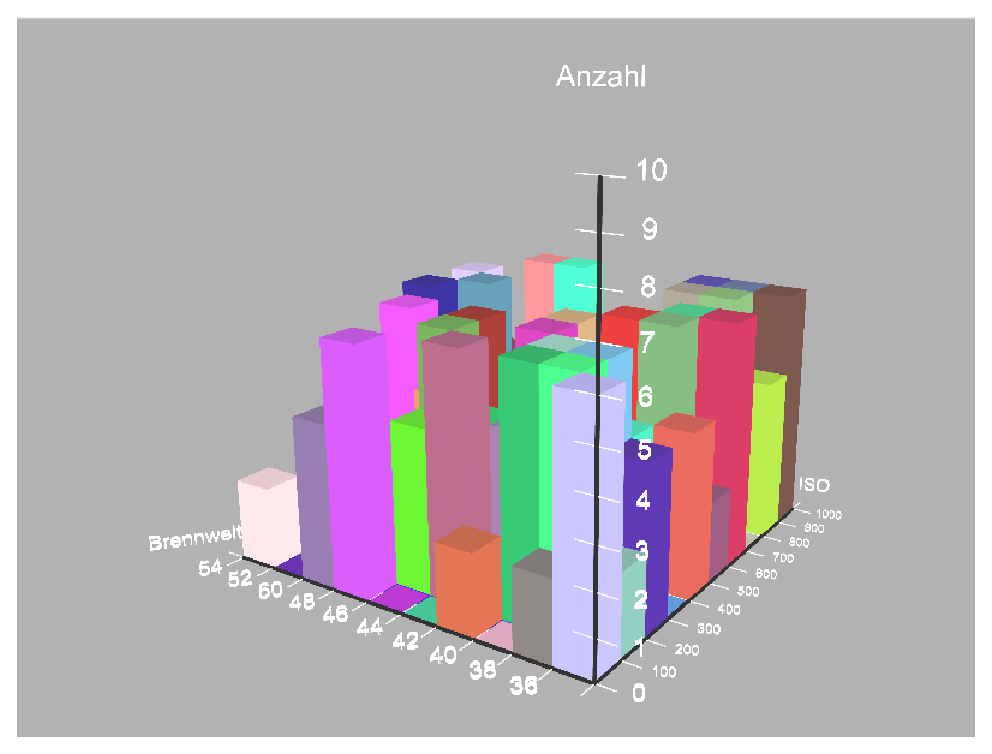
\includegraphics{images/3DHistogramm.eps}
						} 
						\caption{Ansicht eines 3D Histogramms}
						\label{diag:3dhistogramm}
					\end{minipage}  
				}    		
			\end{figure}
			Das 3D Histogramm erlaubt einen weiteren \gls{exif}-Paramter einer zweiten Achse, der z-Achse, zuzuweisen. Dieser muss verschieden von dem \gls{exif}-Paramter der x-Achse sein.
			Dabei wird die xz-Ebene in gleichgroße Rechtecke aufgeteilt. Die y-Achse gibt die Häufigkeit des zu betrachtenden Rechtecks an. Falls n Bildmengen mit der aktuellen Auswertung verbunden sind, so wird jedes Rechteck nochmals in n Rechtecke zerlegt ($ n \in \mathbb{N} $ und $ n>1 $). \par
			
			Die Ansicht kann frei bewegt, rotiert und skaliert werden. Außerdem kann die aktuelle Ansicht durch einen Klick auf die entsprechende Schaltfläche zurückgesetzt werden. Das 3D Histogramm kann als \gls{jpg} via eines Dateidialogs exportiert werden.
\newpage
		\item[/F340/] \textit{Boxplot:}\par 
			\begin{figure}[H]
				\centering
					\fbox{
						\begin{minipage}{13 cm}
							\centering
							% Generated with LaTeXDraw 2.0.2
% Mon Nov 16 01:56:57 CET 2009
% \usepackage[usenames,dvipsnames]{pstricks}
% \usepackage{epsfig}
% \usepackage{pst-grad} % For gradients
% \usepackage{pst-plot} % For axes
\scalebox{1} % Change this value to rescale the drawing.
{
\begin{pspicture}(0,-7.8529)(14.2458,9.8929)
\definecolor{color1297b}{rgb}{0.4980392156862745,0.6705882352941176,1.0}
\definecolor{color1305b}{rgb}{0.9411764705882353,0.6941176470588235,0.08235294117647059}
\psframe[linewidth=0.07,dimen=outer,fillstyle=solid,fillcolor=color1297b](3.8458,2.7929)(2.6458,-3.0071)
\psline[linewidth=0.07cm,tbarsize=0.07055555cm 5.0]{-|*}(3.2458,2.7929)(3.2458,4.8929)
\psline[linewidth=0.07cm,tbarsize=0.07055555cm 5.0]{|-}(3.2458,-5.0071)(3.2458,-3.0071)
\psline[linewidth=0.068cm,linecolor=red](2.7178,-1.2071)(3.7738,-1.2071)
\psdots[dotsize=0.204](3.2458,-0.4071)
\psframe[linewidth=0.07,dimen=outer,fillstyle=solid,fillcolor=color1305b](7.8458,1.8929)(6.6458,-1.6071)
\psline[linewidth=0.07cm,tbarsize=0.07055555cm 5.0]{-|*}(7.2458,1.8929)(7.2458,3.9929)
\psline[linewidth=0.07cm,tbarsize=0.07055555cm 5.0]{|-}(7.2458,-2.7951)(7.2458,-1.5931)
\psline[linewidth=0.068cm,linecolor=red](6.7178,0.4929)(7.7738,0.4929)
\psdots[dotsize=0.204](7.2458,0.6929)
\rput(1.0458,-5.6071){\psaxes[linewidth=0.04,labels=y,ticks=y,ticksize=0.1458cm,dx=1.0cm,dy=0.87cm,Dx=20,Dy=100]{->}(0,0)(0,0)(8,12)}
\usefont{T1}{ptm}{m}{n}
\rput(3.1208,-5.9971){Bildmenge 1}
\usefont{T1}{ptm}{m}{n}
\rput(7.0353312,-5.9971){Bildmenge 2}
\end{pspicture} 
}

							\caption{Ansicht eines Boxplots}
							\label{diag:boxblot}
						\end{minipage}  
					}    		
			\end{figure}
			Der Boxplot stellt einige wesentlichen Beschreibungsmerkmale einer Verteilung in einem Diagramm dar. Dabei wird der Median, hier der rote Balken, der Mittelwert, hier der schwarze Punkt, das untere und obere Quartil dargestellt. Die Whiskers (dt.: Schnurrhaare) zeigen das Maximum beziehungsweise das Minimum einer Verteilung, sofern diese nicht mehr als das 1,5-fache des Interquartilabstands vom Median abweichen. Datenpunkte, die außerhalb dieses Abstandes liegen, gelten als Ausreißer und werden als einzelne Datenpunkte dargestellt.
			\par
			Beim Boxplot können ein bis zwei Bildmengen als Auswertungsgrundlage verwendet werden. Außerdem hat man die Möglichkeit, falls man zwei Bildmengen als Auswertungsgrundlage verwendet, den \gls{wilcoxon} im Einstellungsfenster zu aktivieren (siehe Kapitel \ref{gui:willcoxon}). Dabei muss eine Testart und ein Signifikanzniveau festgelegt werden.
\par Der \gls{wilcoxon} gibt den \gls{pwert} aus. Der Boxplot kann als \gls{jpg} via eines Dateidialogs exportiert werden.

		\item[/F350/] \textit{Punktewolke:}\par		
			\begin{figure}[H]
				\centering
				\fbox{
					\begin{minipage}{13 cm}
						\centering
						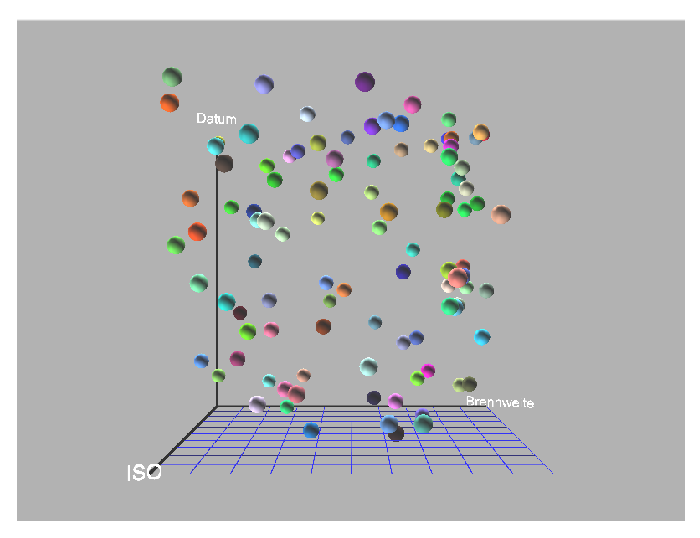
\includegraphics{images/punktewolke.eps} 
      			\caption{Ansicht einer Punktewolke}
      			\label{punktewolke}
					\end{minipage}  
    		}    		
			\end{figure}
			Die Punktewolke ist ein dreidimensionales Diagramm, bei der Punkte in einem kartesisches Koordinatensystem dargestellt werden.
			Dabei können die drei Achsen jeweils mit einem \gls{exif}-Parameter belegt werden, wobei jeder \gls{exif}-Parameter nur einmal verwendet werden darf.
			Punkte, die die gleichen Koordianten haben werden farbkodiert. Eine Farbskala gibt die Häufigkeit der individuellen Punkte an.
			Betätigt man die linken Maustaste auf einem Punkt, so wird das entsprechende Bild als Miniaturansicht mit Namen angezeigt. Verbirgt sich hinter einem Punkt mehrere Bilder, so wird ein beliebiges, aber festes Bild angezeigt. 
			\par 
			
		Die Ansicht kann frei bewegt, rotiert und skaliert werden. Außerdem hat man die Möglichkeit die aktuelle Ansicht mit einem Klick auf die entsprechende Schaltfläche zurückzusetzen.
			Die Punktewolke kann als \gls{jpg} via eines Dateidialogs exportiert werden.

	\end{description}

\subsection{Auswertungsmanagement}

\label{subsec:auswertungsmgmt}

	Eine Auswertung ist eine Verknüpfung von beliebig (im Rahmen der \textbf{/NF020/)} vielen Bildmengen mit einem Diagrammtyp. Eine Auswertung ist dabei folgendermaßen definiert:

	\begin{itemize}

		\item Eine Auswertung kann auch ohne Auswahl von Bildmengen existieren. 

		\item Eine Auswertung hat einen frei definierbaren und vom Projektkontext abhängigen eindeutigen Namen, der zwischen einem und 200 Zeichen lang sein muss.

		\item Eine Auswertung wird über eine interne ID, die innerhalb eines Projekt eindeutig ist, identifiziert.

	\end{itemize}

	Wird ein Projekt geöffnet, werden alle in der Projektkonfigurationsdatei definierten Auswertungen \gls{lexgraph} sortiert angezeigt. Die erste Auswertung der Liste (falls vorhanden), wird dabei automatisch markiert.

	\begin{description}
		
		\item[/F410/] \textit{Anlegen einer neuen Auswertung:}\par Durch betätigen der Schaltfläche "`Erstellen"' in dem Bereich "`Auswertungen"' der Projektansicht, wird ein Assistent gestartet, der den Benutzer durch die Auswertungserstellung führt.\par Über die Schaltfläche "`Vorwärts"' kann der Benutzer dabei auf den nächsten Schritt wechseln, sofern er in der aktuellen Eingabemaske keine Fehleingabe getätigt hat. Durch betätigen der Schaltfläche "`Zurück"', kann der Benutzer hingegen zu einem bereits getätigten Schritt wechseln. Auch hierbei wird vor dem Druck auf "`Vorwärts"' überprüft, ob alle Eingabedaten immer noch korrekt sind.\par Folgende Schritte führt der Assistent aus:

			\begin{enumerate}

				\item \textbf{Diagrammtyp festlegen.}

					\begin{itemize}

						\item Festlegen eines Auswertungsnamens.

						\item Eine optionale Beschreibung der Auswertung.

						\item Auswahl eines Diagrammtyps (siehe Kapitel \ref{subsec:diagrammmgmt}).\par Bei der Auswahl, wird eine Live-Vorschau des Diagramms mit einem Dummy-Datensatz angezeigt, sowie eine kurze Beschreibung über Sinn und Zweck des Diagramms.\par Hier kann auch eine bereits in dem geöffneten Projekt vorhandene Auswertung als Vorlage verwendet werden. Dabei werden alle Werte der Auswertungsvorlage übernommen bis auf die ID und den Namen. Diese beiden Werte müssen neu generiert werden, damit die Definition nicht verletzt wird.

					\end{itemize}

				\item \textbf{Parameter festlegen}.\par Festlegen der x-, y- oder z-Achse (je nach Diagrammtyp - siehe Kapitel \ref{subsec:diagrammmgmt}). Mit Festlegen ist hier das Verknüpfen mit \gls{exif}-Parametern gemeint. Optional kann eine Beschreibung angegeben werden, die dann anstatt der Bezeichnung des \gls{exif}-Parameters verwendet wird.

				\item \textbf{Bildmengen und Filter festlegen}.\par Hier werden Bildmengen des aktuell aktiven Projektes mit der Auswertung verknüpft. Außerdem kann hier anhand der \gls{exif}-Keywords eine Reduzierung der gesamten Bildmenge bewirkt werden. Bei der Zuweisung der Bildmengen mit der aktuellen Auswertung, kann der Benutzer via Schaltflächen Bildmengen der aktuellen Auswertung zuweisen bzw. bereits zugewiesene Bildmengen der aktuellen Auswertung entziehen. 
				
				Zugewiesene Bildmengen, deren Inhalt \gls{exif}-Parameter enthalten, werden in einer weiteren Liste dargestellt.  Dabei werden gleiche \gls{exif}-Keywords zusammengefasst. Bei der Zuweisung der zu verwendenden Filter mit der aktuellen Auswertung, kann der Benutzer via Schaltflächen \gls{exif}-Keywords der aktuellen Auswertung zuweisen bzw. bereits zugewiesene \gls{exif}-Keywords der aktuellen Auswertung entziehen. Als Auswertungsgrundlage werden die Bilder verwendet, die in der Bildmenge vorhanden sind und eines der zugewiesenen \gls{exif}-Keywords besitzen (siehe Kapitel \ref{subsec:benutzerschnittstelle}). 

			\end{enumerate}

			Nach Beendigung des Assistenten durch betätigen der Schaltfläche "`Übernehmen"', wird die Auswertung gespeichert und, falls bereits Bildmengen mit der Auswertung verknüpft wurden, geöffnet.
		
		\item[/F420/] \textit{Markieren einer Auswertung:}\par Um eine Auswertung zu aktivieren, muss man sie in der Liste der Auswertungen im Bereich "`Auswertungen"' der Projektansicht, auswählen.
		
		\item[/F430/] \textit{Bearbeiten einer Auswertung:}\par Um eine Auswertung zu bearbeiten, muss sie markiert sein. Durch betätigen der Schaltfläche "`Bearbeiten"' in dem Bereich "`Auswertungen"' der Projektansicht, wird ein Dialog geöffnet, der die gleichen Auswahlmöglichkeiten des Assistenten aus \textbf{/F310/} enthält. Diese sind über Tabs auswählbar und sind mit den Werten der Auswertung vorbelegt. 
		Durch Klick auf "`Übernehmen"' wird die Änderung aktiv. Mit der Schaltfläche "`Anzeigen"' lässt sich das Resultat der Auswertung begutachten und gleichzeitig das "`Bearbeiten-Fenster"' geschlossen.
		
		\item[/F440/] \textit{Entfernen einer Auswertung:}\par Um eine Auswertung zu entfernen, muss sie markiert sein. Durch betätigen der Schaltfläche "`Entfernen"' in dem Bereich "`Auswertungen"' der Projektansicht, werden folgende Aktionen ausgelöst:

			\begin{enumerate}

				\item Es wird eine Sicherheitsabfrage (ein Dialog mit Ja/Nein Auswahlmöglichkeit) angezeigt, die dem Benutzer die Möglichkeit gibt, das Entfernen abzubrechen.

				\item Die Auswertung wird aus der Liste der Auswertungen entfernt.

				\item Dem Benutzer wird eine Rückmeldung gegeben, ob das Entfernen erfolgreich war oder ob es einen Fehler gab.

				\item Nach dem Entfernen, ist die erste Auswertung (falls vorhanden) in der Liste markiert.

			\end{enumerate}
			
	\end{description}

\subsection{Exif-Auswertung}

	\begin{description}

		\item[/F510/] \textit{Extraktion von \gls{exif}-Parametern:}\par Beim Einlesen von Bildern im \gls{jpg}-Format, werden nur die \gls{exif}-Parameter eingelesen, nicht die Bilddaten. Die \gls{exif}-Parameter, die verarbeitet werden, sind im Kapitel \ref{subsec:musskriterien} definiert. Die Daten werden nur während der Programmausführung intern gespeichert, dies hat zur Konsequenz, dass bei jedem Programmstart, alle \gls{exif}-Parameter neu eingelesen werden müssen (siehe Kapitel \ref{subsec:projektmanagement} \textbf{/F130/}).
	
	\end{description}